\documentclass{article}
%
%
%	LaTeX template
%
%	David Meyer
%	dmm613@gmail.com
%	15 July 2022
%
%
%   get various packages
%
\usepackage[margin=1.0in]{geometry}                                     % adjust margins
\geometry{letterpaper}                                                  % or a4paper or a5paper or ... 
\usepackage{url}                                                        % need this to use URLs in bibtex
\usepackage{setspace}                                                   % need this for \setstrech{...}
\usepackage{scrextend}                                                  % need this for addmargin
\usepackage[export]{adjustbox}                                          % need this to get frame for includegraphics
%
%   tikz et al
%
\usepackage{tikz}
\usetikzlibrary{calc,patterns,angles,quotes,shapes,math,decorations,
                through,intersections,lindenmayersystems,backgrounds,
                hobby}
\tikzset{>=latex}														% default to LaTeX arrow head
\usepackage{circuitikz}                                                 % draw circuits    
\usepackage{pgfplots}
%
%	more math stuff
%
\usepackage{amsmath,amsfonts,amssymb,amsthm}
\usepackage{mathtools}
\usepackage{commath}                                                    % get \norm{x}
\usepackage{fixmath}                                                    % get \mathbold
\usepackage{gensymb}                                                    % get \degree
\usepackage{mathrsfs}
\usepackage{hyperref}
\usepackage{subcaption}
\usepackage{authblk}
\usepackage{graphicx}
\usepackage{hyperref}
\usepackage{alltt}
\usepackage{color}
\usepackage{float}
\usepackage{braket}
\usepackage{siunitx}
\usepackage{relsize}
\usepackage{multirow}
\usepackage{esvect}
%
%	watermarks
%
% \usepackage{draftwatermark}
% \SetWatermarkText{Draft}
% \SetWatermarkScale{5}
% \SetWatermarkLightness {0.9} 
% \SetWatermarkColor[rgb]{0.7,0,0}
%
%
%	theorems, definitions, etc
%
\theoremstyle{definition}
\newtheorem{theorem}{Theorem}[section]
\newtheorem{definition}{Definition}[section]
\newtheorem{proposition}{Proposition}[section]
\newtheorem{lemma}{Lemma}[section]
\newtheorem{example}{Example}[section]
\newtheorem{remark}{Remark}[section]
%
%	The following code allows you to do
%
%	\begin{bmatrix}[r] (or [c] or [l])
%
\makeatletter
\renewcommand*\env@matrix[1][c]{\hskip -\arraycolsep
  \let\@ifnextchar\new@ifnextchar
  \array{*\c@MaxMatrixCols #1}}
\makeatother
%
%	make \arg{min,max}_{n \to \infty} work nicely
%
\newcommand{\argmax}{\operatornamewithlimits{argmax}}
\newcommand{\argmin}{\operatornamewithlimits{argmin}}
%
%	handy commands
%
\newcommand*{\Scale}[2][4]{\scalebox{#1}{$#2$}}
\DeclareMathOperator{\E}{\mathbb{E}}
\DeclareMathOperator{\bda}{\Big \downarrow}						% big down arrow
\newcommand{\veq}{\mathrel{\rotatebox{90}{$=$}}}
%
%	Title, author and date
%

\title{A Few Notes on Projective Geometry (WIP)}
\author{David Meyer \\ \href{mailto:dmm613@gmail.com}
                            {dmm613@gmail.com}}
\date{Last Update: \today \\
	 {\vspace{1.00mm} \small Initial Version: January 15, 2018}}

%
%
%
%
%
%
% \newcommand{\argmin}{\operatornamewithlimits{argmin}}


\begin{document}
\maketitle

\section{Introduction}
These notes began life as a bit of research on elliptic curves. However, it turns out that an elliptic curve is a smooth, projective, algebraic curve of genus one, on which there is a specified point $\mathcal{O}$. An elliptic curve is also abelian in the sense that if it has a multiplication that is defined algebraically, then it is an abelian group with respect to 
this multiplication. In this case $\mathcal{O}$ serves as the identity element. Often the curve itself without $\mathcal{O}$ specified, is called an elliptic curve; the point $\mathcal{O}$ is often taken to be the curve's "point at infinity" in the \emph{projective plane}. 

\bigskip
\noindent
So what is a projective plane? As we will see in Section \ref{sec:projective_plane}, a projective plane is a kind of (projective) geometry. 

\section{The Real Projective Line}
\label{section:real_projective_line}
The real projective line is the set of all lines that pass
through the origin. One way to think about this is as the
one-dimensional subspace of "rays" 
\cite{youtube:vector_spaces_and_quantum_mechanics,wolfram:ray}. 
This is shown on the left in Figure
\ref{figure:real_projective_line_setup}.

\bigskip
\noindent
\setstretch{1.25}{If we slide the red point along the $y = 1$
line in Figure \ref{figure:real_projective_line_setup} the angle
$\theta$ varies between $-\frac{\pi}{2}$ and $\frac{\pi}{2}$ as
$x$ varies between $-\infty$ and $\infty$. In particular, as $x
\to \pm\infty$, $\theta \to \pm \frac{\pi}{2}$.  That is \par}

\begin{equation*}
   \lim\limits_{x \to \infty} \theta = \frac{\pi}{2} 
\end{equation*}
\noindent
and
\begin{equation*}
   \lim\limits_{x \to -\infty} \theta = -\frac{\pi}{2} 
\end{equation*}

\medskip
\noindent
If we then look at the points $(x,\theta)$ you find that the real
projective line can be seen as a circle. This is shown on the
right in Figure \ref{figure:real_projective_line_setup}.
%
%
%	A few parameters
%
\setlength			{\fboxsep} {0.50em}						% space between fcolorbox and content
\setlength			{\fboxrule}{0.75pt}						% fcolorbox line thickness
\def \scalefactor	{1.00}									% resizebox scale factor
\def \minipagescale	{0.50}									% minipage scale factor
\def \twidth		{\textwidth}							% point size of points drawn on the cirle
\def \pointsize		{0.50pt}
%
%	Draw the picture
%
\begin{figure}[H]
\centering
\fcolorbox{black}{white} {
  \begin{minipage}[t]{\minipagescale \textwidth}
    \centering
    \resizebox{\scalefactor \textwidth}{!}{
      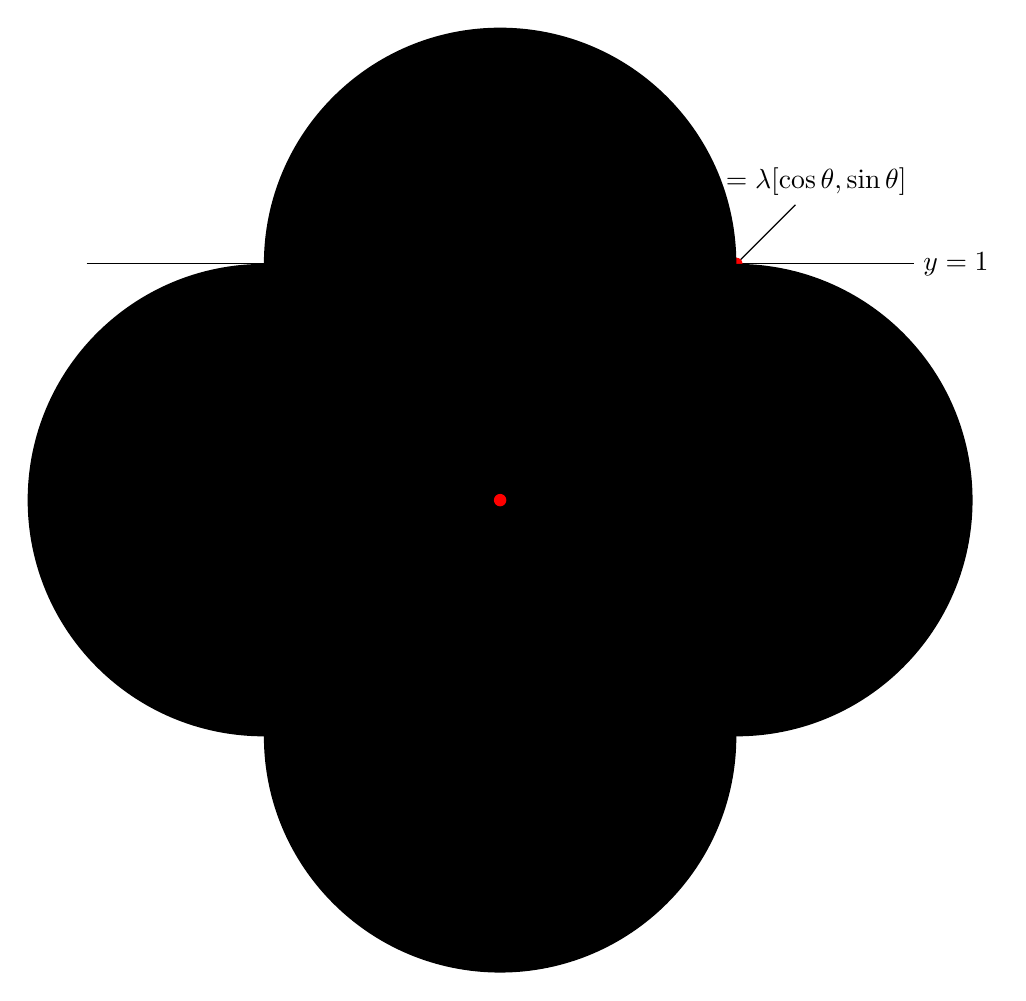
\begin{tikzpicture}[scale=3]
      % Draw the axes
        \draw[-] (-1.75,0) -- (1.75,0) node[below,xshift=-0.15cm]               {$x$};
        \draw[]  (1.50,0)              node[above,xshift=0.25cm]                {$\lambda[1,0]$};
        \draw[-] (0,-0.50) -- (0,1.50) node[right,xshift=0.20cm,yshift=-0.20cm] {$y$};
        \draw[]  (0,1.50)              node[above]                              {$\lambda[0,1]$};
        % Draw the y = 1 line
        \draw [-] (-1.75,1) -- (1.75,1);
        % Draw the y = x line
        \draw [-] (-1.00,-1.00) -- (1.25,1.25) node[above,xshift=-0.25cm] 
        		{$\lambda[x,1] = \lambda [\cos \theta, \sin \theta]$};
        % Intersection of y = 1 and y = x
        \fill [red] (1,1) circle (0.75pt);
        \node [below,yshift=-0.1cm,xshift=0.25cm] at (1,1) {$(1,\frac{\pi}{4})$};
                \node [right,xshift=-0.75cm] at (2,1) {$y = 1$};
        % Draw theta
        \draw [<-] (0.3,0.3) arc (45:90:0.42);
        \node[] at (0.10,0.25) {$\theta$};
        % Draw upper half of unit circle in blue
        \draw [blue,thick] (1,0) arc (0:180:1);
        % Draw bottom half of unit circle in dashed black
        \draw [dashed,thick](-1,0) arc (180:360:1);
        % Put some black points on the unit circle
        \fill [black] (1,0)  circle (\pointsize); 
        \fill [black] (-1,0) circle (\pointsize); 
        \fill [black] (0,1)  circle (\pointsize);
        \fill [black] (0,-1) circle (\pointsize);
        % Draw a dot at the origin
        \fill [red] (0,0) circle (0.75pt);
        % Draw a few coordinates of interest
        \draw (1,0)  node[below]                {$(1,0)$};
        \draw (-1,0) node[below]                {$(-1,0)$};
        \draw (0,1)  node[below,yshift=-0.10cm] {$(0,1)$};
        \draw (0,-1) node[below]                {$(0,-1)$};
      \end{tikzpicture}
      }
  \end{minipage}

%
%	Force the figures to be side by side
%
  \hfill
%
%	Scale the second image
%  
\def \scalefactor {0.775}
\def \minipagescale	{0.50}									% minipage scale factor

%
%	Draw the second figure
%
   \begin{minipage}[t]{\minipagescale \textwidth}
     \centering
     \resizebox{\scalefactor \textwidth}{!}{
        
\begin{tikzpicture}[scale=3]
           \draw [blue,thick] (0,0) circle (1); 
           \node[right,xshift=0.20cm] at (1,0) {$(1,\frac{\pi}{4})$};
           \node[above] at (0,1) {$(0,0)$};
           \node[left,xshift=-0.20cm] at (-1,0) {$(-1,-\frac{\pi}{4})$};
           \node[below,yshift=-0.15cm] at (0,-1) {$(-\infty,-\frac{\pi}{2};\infty,\frac{\pi}{2})$};
           \node[] at (1,1) {$\mathbf{(x},\boldsymbol{\theta}\mathbf{)}$};
           \fill [black] (1,0)  circle (\pointsize); 
           \fill [black] (0,1)  circle (\pointsize); 
           \fill [black] (-1,0) circle (\pointsize);
           \fill [black] (0,-1) circle (\pointsize); 
       \end{tikzpicture}
     }
   \end{minipage}
  }
  \caption{Real Projective Line Setup}
  \label{figure:real_projective_line_setup}    
\end{figure}
%
%
%
\section{Geometries and Projective Planes}
\label{sec:projective_plane}
In this section we will start by defining what a Geometry is and look at a few examples.

\begin{definition} \textbf{(Geometry):} A geometry $S = (P, L)$ is a non-empty set $P$ whose elements are called \emph{points} together with a set $L$ of 
non-empty subsets of $P$ called \emph{lines} which satisfy:
\begin{itemize}
\item G1: For any two distinct points $p_1,p_2 \in P$, there exists exactly one line $l \in L$ such that both $p_1 \in l$ and $p_2 \in l$.
\item G2: There exists a set of four points, such that given any set of three of these points, no line exists that contains all three points.
\end{itemize}

\noindent
Note that $P$ and $L$ may be either finite or infinite. We say that a point $p$ is on, or \emph{incident with} $p$ if $p \in l$. 
In the same way a line $l$ is on or \emph{incident with} a point $p$ if $p \in l$. 

\noindent
A set of points is called \emph{collinear} if there exists a line such that all points are on the line. If $p$ and $q$ are two points, then $pq$ denotes the 
unique line on both $p$ and $q$. Clearly $qp = pq$. If $l_1$ and $l_2$ are lines that intersect in a point, $l_1l_2$ denotes their point of intersection.

\noindent
Using this notation, we can write G1 and G2 in a more concise way way: 
\begin{itemize}
\item G1: Two distinct points are on exactly one line.
\item G2: There exists a set of four points, no three of which are collinear.
\end{itemize}

\noindent
A set of four points, no three of which are collinear, is called a \emph{quadrangle}. A line through two points of a quadrangle is called a \emph{diagonal}
of the quadrangle.
\end{definition}

\begin{example}
This Euclidean plane is a geometry. Why? Well, in the Euclidean plane the set $P$ consist of $(x,y)$ points and the set $L$ consists lines of the
form $y = mx + b$. Also, it is a well-known that two points are on a unique line in the Euclidean plane, so G1 holds.  In addition, the set  $\{(0,0), (1,0), (0,1), (1,1)\}$ 
form a quadrangle and so G2 holds. 
So the Euclidean plane is a geometry.
\end{example}

\begin{lemma} Two distinct lines in a geometry intersect in at most one point.
\end{lemma}

\noindent
\textbf{Proof.} Assume that there are two lines that intersect in at least two points, and let two such points be $p_1$ and $p_2$. But by G1
there is exactly one line on both $p_1$ and $p_2$ and so our assumption is contradicted. So two distinct lines in a geometry intersect in at 
most one point.

\begin{definition} \textbf{(Affine Plane):}  An affine plane is a geometry that satisfies the following condition: 
\begin{itemize}
\item AP: For any line $l$ and any point $p$ not on $l$, there exists a unique line $l^\prime$ on $p$ that does not intersect $l$.
\end{itemize}
This is the famous parallel axiom of Euclidean geometry. Clearly, the Euclidean plane is an affine plane. The obvious connection to the
 parallel axiom justifies the following definition.
\end{definition}

\begin{definition}  \textbf{(Parallel Lines):}. Two lines in an affine planes are said to be parallel if they do not intersect. Any line is also said to be parallel to itself.
If $l_1$ and $l_2$ are two parallel lines we write $l_1 \parallel l_2$.
\end{definition}

\begin{lemma} The relation "is parallel" on the lines of an affine plane $A$ is an equivalence relation.
\end{lemma}

\noindent
\textbf{Proof.}  Let $l_1,l_2$ and $l_3$ be three distinct lines of $A$. Then

\begin{itemize}
\item By definition $l_1 \parallel l_1$ so $\parallel$ is reflexive. 
\item Assume that $l_1 \parallel l_2$, Then $l_2$ does not intersect $l_1$ either, so $l_2 \parallel l_1$ and so $\parallel$  is symmetric. 
\item Finally, to show transitivity  assume that $l_1 \parallel l_2$ 
and $l_2 \parallel l_3$, but $l_1 \nparallel l_3$. Then $l_1$ and $l_3$ intersect in a point $p$. But then $p$ is on two lines ($l_1$ and $l_3$) but not on $l_2$.
This contradicts AP since AP says there is a \emph{unique} parallel line and here we have two. Hence  $l_1 \parallel l_3$, and so $\parallel$  is transitive. 
$\blacksquare$
\end{itemize}

\bigskip
\noindent
The equivalence relation "is parallel" is kind of interesting in that it partitions the set of lines in an affine plane into parallel classes. So for a line $l$ in an affine plane, 
we denote its parallel class by $[l]$. $[l]$ consists of all lines parallel to $l$.

\begin{lemma} Let $p$ be a point of an affine plane. For each parallel class of lines, there is exactly one line on $p$ that belongs to the class.
\end{lemma}

\noindent
\textbf{Proof.} Let [l] be any parallel class for $l \in L$. If $l$ is not on $p$ then by AP there exists a unique line on $p$ parallel to $l$ so done. 
If $l$ is on $p$, we must show that no other line on $p$ is also in $[l]$. But any other line on $p$ intersects $l$ at $p$, so the lines are not parallel.
$\blacksquare$

\bigskip
\noindent
Ok, but what is a projective plane?

% \newpage

\subsection{Projective Planes}
\begin{definition} \textbf{(Projective plane): } A projective plane is a geometry that satisfies the following condition:
\begin{itemize}
\item PP: Any two lines intersect in exactly one point.
\end{itemize}
\end{definition}

\noindent
So what is the difference between affine and projective planes?  In an affine plane parallel
lines exists whereas in projective planes two unique lines always intersect (at one point).

\subsection{The Fano Plane}
\label{subsec:fano_plane}
The Fano Plane, named for Italian mathematician Gino Fano  \cite{wiki:gino_fano}, is the finite projective plane of order 2. It is the finite projective plane with the \emph{smallest 
possible number of points and lines}: 7 points and 7 lines, with 3 points on every line and 3 lines through every point. The standard notation for this plane, 
as a member of a family of projective spaces, is PG(2, 2) where PG stands for "projective geometry", the first parameter is the geometric dimension and 
the second parameter is the order.

\bigskip
\noindent
More precisely, let $\Pi = (P,L)$ be a geometry where $P = \{1,2,3,4,5,6,7\}$ and $L = \{l_1,l_2,l_3,l_4,l_5,l_6,l_7\}$ and let 
$l_1 = \{1,2,3\}, \:  l_2 = \{1,4,5\}, \:  l_3 = \{1,6,7\}, \: l_4 = \{2,4,6\},  \: l_5 = \{2,5,7\},  \: l_6 = \{3,4,7\}$ and $l_7 = \{3,5,6\}$. This labelling
is shown in Figure \ref{fig:fano_plane}. Here $\Pi$  is a projective plane as it easily satisfies G1 and PP and  $\{1, 2, 4, 7\}$ is an example 
of a quadrangle on $\Pi$.

\bigskip
\noindent
Legend has it that the Fano Plane was invented as a solution to a game posed by Fano. The challenge was to create a projective 
plane with the smallest possible number of points and lines, 7 each, with 3 points on every line and 3 lines through every point. 
The problem remained unsolved until someone observed that not all lines need be straight. A circle was then added to the projective plane to create what we know
 as the Fano Plane today. The Fano Plane shown in Figure \ref{fig:fano_plane}.

\bigskip
\begin{figure}[H]
\center{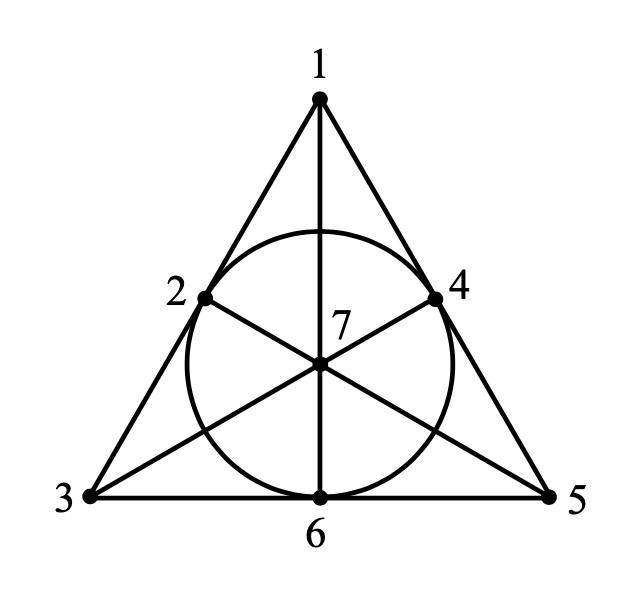
\includegraphics[scale=0.4] {images/fanoplane.jpg}}
\caption{The Fano Plane}
\label{fig:fano_plane}
\end{figure}


\section {Homogeneous Coordinates}
Homogeneous Coordinates are a convenient way to represent translations and rotations which allows them both to be expressed as a matrix multiplication. This has certain computational and notational conveniences, and eventually leads us to a wider and interesting class of transformations. 

\bigskip
\noindent
Suppose we wish to translate all points $(X, Y, Z)$ by adding some constant vector $(t_x, t_y, t_z)$ to all coordinates. One way to accomplish this is to embed 
the points $(X, Y, Z) \in \mathbb{R}^3$ in $\mathbb{R}^4$ by tacking on a fourth coordinate with value 1. So the embedding of $\mathbb{R}^3$ in 
$\mathbb{R}^4$ looks like

\bigskip
\begin{equation*}
\begin{bmatrix} X \\ Y \\ Z  \end{bmatrix} \hookrightarrow \begin{bmatrix} X \\ Y \\ Z \\ 1 \end{bmatrix} 
\end{equation*}

\bigskip
\noindent
So we want the translated point

\begin{equation*}
\begin{bmatrix} X + t_x \\ Y + t_y \\ Z + t_z \\ 1 \end{bmatrix} 
\end{equation*}


\bigskip
\noindent
We can get this translation by multiplying by a "translation matrix"

\begin{equation*}
\begin{bmatrix}  1 & 0 & 0 & t_x \\ 
                          0 & 1 & 0 & t_y \\ 
                          0 & 0 & 1 & t_z \\
                          0 & 0 & 0 & 1     \\
\end{bmatrix} 
\end{equation*}


\bigskip
\noindent
Then the translation, represented as matrix multiplication, looks like


\begin{equation*}
\begin{bmatrix}  1 & 0 & 0 & t_x \\ 
                          0 & 1 & 0 & t_y \\ 
                          0 & 0 & 1 & t_z \\
                          0 & 0 & 0 & 1     \\
\end{bmatrix} 
\begin{bmatrix} X \\ Y \\ Z \\ 1 \end{bmatrix} =
\begin{bmatrix*}[l]
1 \cdot X  &+& 0 \cdot Y &+& 0 \cdot Z   &+&  t_x \cdot 1 \\
0 \cdot X  &+& 1 \cdot Y  &+& 0 \cdot Z  &+&  t_y \cdot 1\\
0 \cdot X  &+& 0 \cdot Y  &+& 1 \cdot Z  &+&  t_z \cdot 1\\
0 \cdot X  &+& 0 \cdot Y  &+& 0 \cdot Z   &+& 1 \cdot 1
\end{bmatrix*} =
\begin{bmatrix} X + t_x \\ Y + t_y \\ Z + t_z \\ 1 \end{bmatrix} 
\end{equation*}

\bigskip
\noindent
We can perform rotations using a $4 \times 4$ matrix as well. Rotations matrices go into the upper-left
$3 \times 3$ corner of the $4 \times 4$ matrix

\begin{equation*}
\begin{bmatrix}  * & * & * & 0 \\ 
                          * & * & *  & 0 \\ 
                          * & * & * & 0 \\
                          0 & 0 & 0 & 1     \\
\end{bmatrix} 
\end{equation*}

\bigskip
\noindent
We can also scale the three coordinates with a scaling matrix


\begin{equation*}
\begin{bmatrix}  \sigma_x & 0 & 0 & 0 \\ 
                          0 & \sigma_y& 0 & 0 \\ 
                          0 & 0 & \sigma_z & 0 \\
                          0 & 0 & 0 & 1     \\
\end{bmatrix} 
\end{equation*}

\bigskip
\noindent
so that 

\begin{equation*}
\begin{bmatrix}  \sigma_x & 0 & 0 & 0 \\ 
                          0 & \sigma_y& 0 & 0 \\ 
                          0 & 0 & \sigma_z & 0 \\
                          0 & 0 & 0 & 1     \\
\end{bmatrix} 
\begin{bmatrix} X \\ Y \\ Z \\ 1 \end{bmatrix} =
\begin{bmatrix*}[l]
\sigma_x  \cdot X  &+&  0             \cdot Y    &+& 0 \cdot Z                &+& 0 \cdot 1 \\
0 \cdot X               &+&  \sigma_y \cdot Y    &+& 0 \cdot Z                &+& 0 \cdot 1 \\
0 \cdot X               &+& 0               \cdot Y    &+& \sigma_z \cdot Z   &+& 0 \cdot 1 \\
0 \cdot X              &+& 0                \cdot Y    &+& 0 \cdot Z               &+& 1 \cdot 1
\end{bmatrix*} =
\begin{bmatrix} \sigma_x X \\ \sigma_y Y \\ \sigma_z Z \\ 1 \end{bmatrix} 
\end{equation*}

\bigskip
\noindent
So far we have represented (embedded) points $(X, Y, Z) \in \mathbb{R}^3$ as points $(X, Y, Z, 1) \in \mathbb{R}^4$. We can generalize this by representings
the points $(X, Y, Z) \in \mathbb{R}^3$ as \emph{any} vector of the form $(wX, wY, wZ, w) \in \mathbb{R}^4$, where $w \neq 0$. Note that the set of points

\bigskip
\begin{equation*}
\big \{(wX,wY,wZ,w) \mid w \neq 0\big \}
\end{equation*}

\bigskip
\noindent
is a line in $\mathbb{R}^4$  that passes through the origin and the point $(X,Y,Z,1)$. 

\bigskip
\noindent
Here we are associating each point  $(X,Y,Z) \in \mathbb{R}^3$ with a line in $\mathbb{R}^4$ that passes through the origin. 
This representation is called \emph{homogeneous coordinates}.

\bigskip
\noindent
BTW is this generalization consistent with the $4 \times 4$ rotation, translation, and scaling matrices above? It turns out that it is. This is because
for any $\mathbf{X} = (X, Y, Z, 1)$ and \emph{any} $4 \times 4$ matrix $\mathbf{M}$ we have

\begin{equation*}
w(\mathbf{MX}) \equiv \mathbf{M}(w\mathbf{X})
\end{equation*}

\bigskip
\noindent
That is, multiplying each component of the vector $\mathbf{X}$ by $w$ and then transforming by $\mathbf{M}$ yields the same vector as transforming 
$\mathbf{X}$ itself by $\mathbf{M}$ and then muliplying each component of $\mathbf{MX}$ by $w$. But multiplying each component of $\mathbf{X}$
by $w$ doesn?t change how that vector is transformed.

\bigskip
\noindent
There is another way do define homogeneous coordinates in terms of the \emph{Real Projective Plane}. Before being able to do this however we need 
a few definitions.

\begin{definition} {\bf (Real Projective Plane):}
The real projective plane is the space of equivalence classes

\begin{equation*}
\mathbb{R}P^2 =  \{\mathbb{R}^3 \backslash (0,0,0) \} / \sim
\label{eqn:rpp}
\end{equation*}

\bigskip
\noindent
where $\sim$ is the equivalence relation such that $(x_1,y_1,z_1) \sim (x_2,y_2,z_2)$
if $\exists t \neq 0$ such that $x_2 = t \cdot x_1$, $y_2 = t \cdot y_1$, and $z_2 = t \cdot z_1$.
\end{definition}

\bigskip
\noindent
Then the alternate definition of  homogeneous coordinates is

\begin{definition} {\bf Homogeneous Coordinates:}
The points of $\mathbb{R}P^2$ are called homogeneous coordinates: $[x \mathord{:} y \mathord{:} z]$, where the colons indicate that the \emph{ratios}
between the coordinates are the only things that are significant (recall that the notation $[x]$ refers to the equivalence class of $x$).
\end{definition}

\bigskip
\noindent
We can generalize this definition as follows

\begin{definition} {\bf Projective Spaces:} The projective spaces 

\begin{equation*}
\mathbb{R}P^n = \{\mathbb{R}^{n+1} \backslash \text{Origin}\} / \sim 
\end{equation*}

and
\begin{equation*}
\mathbb{C}P^n = \{\mathbb{C}^{n+1} \backslash \text{Origin}\} / \sim 
\end{equation*}

\bigskip
\noindent
are sets of equivalence classes via an $n + 1$-dimensional version of
Equation \ref{eqn:rpp} where $t$ is in $\mathbb{R}$ and $\mathbb{C}$ 
respectively.
\end{definition}

\bigskip
\noindent
These projective spaces can be broken down into unions of ordinary Euclidean space and other projective spaces. For example:

\begin{proposition} {\bf Inclusions:} We have the following inclusions 
\begin{equation*}
(x_1, \cdots, x_n) \mapsto [x_1 \mathord{:} \cdots \mathord{:} x_n \mathord{:} 1]
\end{equation*}
\begin{equation*}
\mathbb{R}^n  \hookrightarrow \mathbb{R}P^n
\end{equation*}
\begin{equation*}
\mathbb{C}^n  \hookrightarrow \mathbb{C}P^n
 \end{equation*}
 
\bigskip
\noindent
This means that a point $[x_1:\hdots: x_{n+1}] \in \mathbb{C}P^n$ with $x_{n+1} \neq 0$ corresponds to the point

\bigskip
\begin{equation*}
\Bigg (  \frac{x_1}{x_{n+1}}, \hdots, \frac{x_n}{x_{n+1}} \Bigg ) \in \mathbb{C}^n
\end{equation*}

\bigskip
\noindent
We also have

\begin{equation*}
[x_1 \mathord{:}   \cdots \mathord{:} x_n] \mapsto [x_1 \mathord{:}  \cdots \mathord{:}  x_n \mathord{:} 0]
\end{equation*}
\begin{equation*}
\mathbb{R}P^{n-1}  \hookrightarrow \mathbb{R}P^n
\end{equation*}
\begin{equation*}
\mathbb{C}P^{n-1}  \hookrightarrow \mathbb{C}P^n
 \end{equation*}
 
 \bigskip
 \noindent
 and
 \begin{equation*}
\mathbb{R}P^n  = \mathbb{R}^n \cup \mathbb{R}P^{n-1}
\end{equation*}
\begin{equation*}
\mathbb{C}P^n  = \mathbb{C}^n \cup \mathbb{C}P^{n-1}
 \end{equation*}
 
 \bigskip
 \noindent
where the embedded copies of $\mathbb{R}P^{n - 1}$ and $\mathbb{C}P^{n - 1}$ are called the "spaces at infinity" and 
every point, $[x_1 \mathord{:}  \cdots \mathord{:}   x_{n+1}] \in \mathbb{C}P^n$ is either in the image of $\mathbb{C}^n$ (if $x_{n+1} \neq 0$) 
or in the image of $\mathbb{C}P^{n - 1}$ (if $x_{n + 1} = 0$).
\end{proposition}

\bigskip
\noindent
It looks like reason for the term "space at infinity" is that the point $[x_1:\hdots:x_{n+1}] \in \mathbb{C}P^n$ with $x_{n+1} \neq 0$ corresponds to the point


\bigskip
\begin{equation*}
\Bigg (  \frac{x_1}{x_{n+1}}, \hdots, \frac{x_n}{x_{n+1}} \Bigg ) \in \mathbb{C}^n
\end{equation*}

\bigskip
\noindent
and this point moves out to infinity as $x_{n+1} \to 0$. 

\bigskip
\noindent
Another way to think about this is that so far we have considered points like $(wX,wY,wZ,w)$ under the condition that $w \neq 0$ 
and where this point  is associated with $(X,Y,Z) \in \mathbb{R}^3$. So what happens if we let $w = 0$? To understand this consider the point 
$(X, Y, Z, \epsilon) \in \mathbb{R}^4$ where $\epsilon > 0$ and so

\begin{equation*}
(X,Y,Z,\epsilon) \equiv  \bigg ( \frac{X}{\epsilon}, \frac{Y}{\epsilon}, \frac{Z}{\epsilon}, 1 \bigg )
\end{equation*}

\bigskip
\noindent
Now, if we let $\epsilon \to 0$  then the corresponding point $(\frac{X}{\epsilon} , \frac{Y}{\epsilon} , \frac{Z}{\epsilon} )$ goes to infinity while staying along the line 
from the origin through the point $(X, Y, Z, 1)$. As a result we identify the limit $(X, Y, Z, 0)$ with a point at infinity, namely 

\bigskip
\begin{equation*}
(X, Y, Z, 0) \coloneqq \lim_{\epsilon \to 0} \bigg  (\frac{X}{\epsilon} , \frac{Y}{\epsilon} , \frac{Z}{\epsilon} \bigg )
\end{equation*}

\begin{figure}
\center{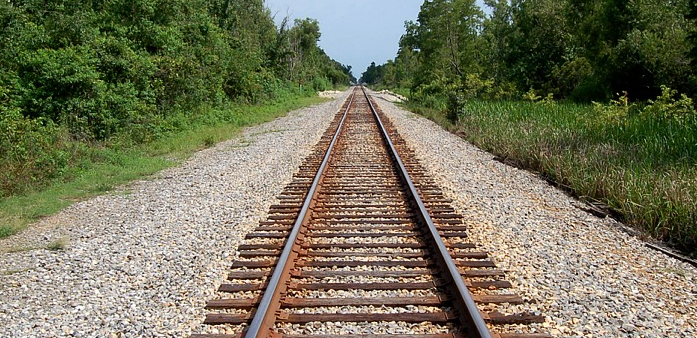
\includegraphics[scale=0.50,frame] {images/parallel_lines.png}}
\caption{Why do parallel lines appear to intersect in the distance?}
\label{fig:parallel_lines}
\end{figure}

\bigskip
\noindent
One other perhaps reassuring way to think about this: consider that parallel lines appear to intersect in the far distance as shown in Figure \ref{fig:parallel_lines} and
that the equation for a single line is

\begin{equation}
y = ax + b
\label{eqn:line}
\end{equation}

\bigskip
\noindent
We can rewrite Equation \ref{eqn:line} as 

\begin{equation*}
x_2 = a_1 x_1 + b_1
\end{equation*}

\bigskip
\noindent
In this case we have points $(x_1,x_2) \in \mathbb{C}^2$ gives rise to homogeneous coordinates $[x_1 \mathord{:}   x_2 \mathord{:}   x_3]$
in $\mathbb{C}P^2$ where

\bigskip
\begin{equation*}
(x_1,x_2) \mapsto [x_1  \mathord{:}  x_2  \mathord{:}  x_3] \Rightarrow \\
(x_1,x_2) \mapsto  \bigg [ \frac{x_1}{x_3}  \mathord{:}  \frac{x_2}{x_3}  \mathord{:}  1 \bigg ]
\end{equation*}

\bigskip
\noindent
and so

\bigskip
\begin{equation*}
\frac{x_2}{x_3} = a_1 \frac{x_1}{x_3} + b_1
\end{equation*}

\bigskip
\noindent
or 
\begin{equation}
x_2 = a_1 x_1 + b_1 x_3
\label{eqn:projective_line}
\end{equation}


\bigskip
\noindent
So we can see that lines in $\mathbb{C}^2$ map uniquely to lines in $\mathbb{C}P^2$ by Equation \ref{eqn:projective_line}. So here's a proposition:


\bigskip
\begin{proposition} Two \emph{distinct} lines
\begin{flalign*}
x_2 &= a_1 x_1 + b_1 x_3   \\
x_2 &= a_2 x_1 + b_2 x_3
\end{flalign*}

\bigskip
\noindent
in $\mathbb{C}P^2$ intersect in one point. If they are parallel (that is, $a_1 = a_2 = a$) then they intersect
at the point $[x_1  \mathord{:}  ax_1  \mathord{:}  0]$. That is, at infinity. 

\bigskip
\noindent
{\bf Proof.}  If the lines are not parallel (i.e., $a_1 \neq a_2$) then they intersect in $\mathbb{C}^2 \subset \mathbb{C}P^2$ in the usual way.
If $a_1 = a_2 = a$, then

\begin{equation*}
\begin{array}{llll} 
  & x_2 &=& a x_1 + b_1 x_3   \\
- &x_2 &=& a x_1 + b_2 x_3   \\
\hline                                       
& 0 &=& 0 + (b_1 - b_2) x_3
\end{array}
\end{equation*}

\bigskip
\noindent
So $0 = 0 + (b_1 - b_2) x_3 \Rightarrow 0 = (b_1 - b_2) x_3$. Since the two lines were distinct but parallel we know that $b_1 \neq b_2 \Rightarrow b_1 - b_2 \neq 0$, So
$x_3$ must be zero which implies that  $x_2 = a x_1 + b \cdot 0$ or $x_2 = ax_1$.  Then the original two lines intersect at the point
$[x_1  \mathord{:}   ax_1  \mathord{:}   0] \in \mathbb{C}P^1 \subset \mathbb{C}P^2$. That is, at infinity. $\blacksquare$
\end{proposition}



\bigskip
\noindent
A question we might ask is what happens to a point at infinity when we perform a rotation, translation, or scaling? Since the bottom row of each of these 
$4 \times 4$ matrices is $(0,0,0,1)$, it is easy to see that these transformations map points at infinity to points at infinity. In particular,

\begin{itemize}
\item A translation matrix does not affect a point at infinity; i.e. it behaves the same as the identity matrix.
\item A rotation matrix maps a point at infinity in exactly the same way it maps a finite point, namely, $(X,Y,Z,1)$ rotates to 
$(X^\prime,Y^\prime,Z^\prime,1)$ if and only if $(X,Y,Z,0)$ rotates to $(X^\prime,Y^\prime,Z^\prime,0)$.
\item A scale matrix maps a point at infinity in exactly the same way it maps a finite point, namely, $(X, Y, Z, 1)$ maps to 
$(\sigma_x X, \sigma_y Y, \sigma_z Z, 1)$ if and only if $(X, Y, Z, 0)$ scales to $(\sigma_x X, \sigma_y Y, \sigma_z Z, 0)$.
\end{itemize}


\noindent
We sometimes interpret points at infinity as \emph{direction} vectors, that is, they have a direction but no position. One must be careful in refeing to them in this way, though, since vectors have a length whereas points at infinity $(X, Y, Z, 0)$ do not have a length.
\section{Conclusions}
%
%
%
\section{Acknowledgements}
%
%	LaTeX source on overleaf.com
%
\section*{\LaTeX \hspace{0.10 mm} Source}
% \url{}
%
%	get a bibliography
%
%	Note:.bib files go in ~/Library/texmf/bibtex/bib with TeXShop (MacTeX).
%	You can also use an absolute path, e.g. \bibliography{/Users/dmm/papers/bib/qc}
%
\bibliographystyle{plain}
\bibliography{qc}
%
%	done
%
\end{document} 
